\documentclass{beamer}
\usepackage[utf8]{inputenc}
\usepackage{xcolor}
\usepackage{enumitem}
\usepackage{listings}
\usepackage{tikz}
\usepackage{tikzsymbols}

% Configuring tikz style
\usetikzlibrary{shapes.geometric, shapes.symbols, arrows}
\tikzstyle{process} = [signal,  text width=1.5cm, minimum height=1.5cm,text centered, draw=black, fill=green!30]
\tikzstyle{maybe} = [signal,  text width=1.5cm, minimum height=1.5cm,text centered, draw=black ]

% Configuring lstlisting code style
\definecolor{codegreen}{rgb}{0,0.6,0}
\definecolor{codegray}{rgb}{0.5,0.5,0.5}
\definecolor{backcolour}{rgb}{0.95,0.95,0.92}

\lstdefinestyle{mystyle}{
  backgroundcolor=\color{backcolour},
  commentstyle=\color{codegreen},
  keywordstyle=\color{ctcorange},
  numberstyle=\tiny\color{codegray},
  stringstyle=\color{purple},
  basicstyle=\ttfamily\footnotesize\tiny,
  captionpos=b,
  keepspaces=true,
  numbers=left,
  numbersep=5pt,
}

% Configuring protobuf code coloring style
\lstdefinelanguage{protobuf}{
    keywords={import, message, enum, syntax, option, repeated, reserved},
    morecomment=[s][\color{ctcorange}]{string}{\ },
    sensitive=false, % keywords are not case-sensitive
    morecomment=[l]{//}, % l is for line comment
    morestring=[b]" % defines that strings are enclosed in double quotes
} %
\lstset{style=mystyle}

% Configuring Camptocamp colors
\usetheme{default}
\definecolor{ctcorange}{HTML}{FF680A}
\definecolor{ctcgray}{HTML}{7A7F82}
\setbeamercolor*{palette primary}{use=structure,fg=ctcorange,bg=white}
\setbeamercolor{titlelike}{parent=ctcorange,fg=structure.fg!50!black}
\setbeamercolor{frametitle}{bg=ctcgray!10!white,fg=ctcorange}
\setbeamercolor*{titlelike}{parent=palette primary}

\title{Data Serialization with Protocol Buffers}
\author{Andrey Rusakov}
\date{\today}

\def\code#1{\texttt{#1}}

\begin{document}

\begin{frame}
\titlepage
\end{frame}

% Introduction
\begin{frame}{Introduction}
\centering
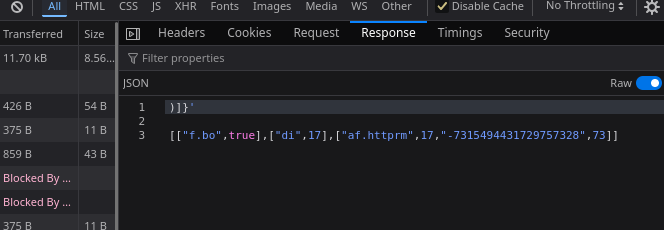
\includegraphics[width=5cm]{gmail-proto}
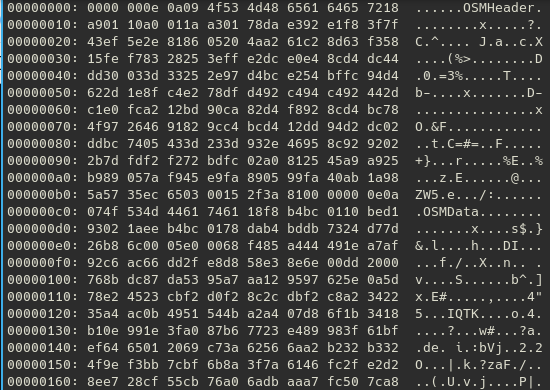
\includegraphics[angle=45,width=4cm]{planet-header}
\end{frame}

% Size comparisons
\begin{frame}[fragile]{Protobuf pipeline}
  \begin{center}
    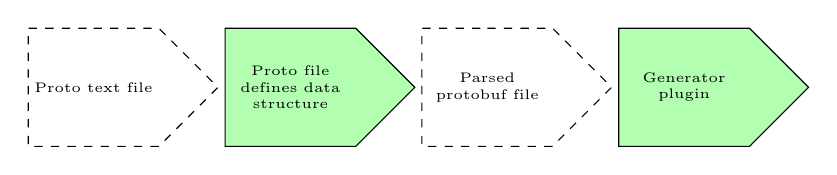
\begin{tikzpicture}[node distance=2.5cm]\tiny
      \node (proto) [maybe, dashed] {Proto text file };
      \node (compiler) [process, right of=proto] {Proto file defines data structure};
      \node (parsed) [maybe, dashed, right of=compiler] {Parsed protobuf file };
      \node (lang) [process, right of=parsed] {Generator plugin};
    \end{tikzpicture}
  \end{center}
\end{frame}

\begin{frame}[fragile]{Proto file: Syntax}
\begin{lstlisting}[language=protobuf, caption={Typical protocol buffer file}]
syntax = "proto3";
option go_package = "demo/proto";

// Message
message Polygon {
  // Nested message with scalar field
  message Point {
    double x = 1;
    double y = 2;
  }
  // Repeated field (list)
  repeated Point vertex = 1;
  string epsg = 2;
}

// Enum definition
enum AreaType {
  UNKNOWN = 0;
  PUBLIC = 1;
  PRIVATE = 2;
}

message Area {
   repeated Polygon polygons = 1;
   AreaType areaType = 2;

  // Reserved fields
  reserved "location", "owner";
}
\end{lstlisting}
\end{frame}

\begin{frame}[fragile]{Parsed proto file}
\begin{lstlisting}[language=protobuf, caption={Parsed protobuf file}]
file_to_generate: "schema.proto"
compiler_version {
  major: 6
  minor: 31
  patch: 0
  suffix: "-dev"
}
proto_file {
  name: "schema.proto"
  package: "example"
  message_type {
    name: "Polygon"
    field {
      name: "points"
      number: 1
      label: LABEL_REPEATED
      type: TYPE_MESSAGE
      type_name: ".example.Polygon.Point"
      json_name: "points"
    }
    field {
      name: "epsg"
      number: 2
      label: LABEL_OPTIONAL
      type: TYPE_STRING
      json_name: "epsg"
    }
\end{lstlisting}
\end{frame}

% Codegen
\begin{frame}[fragile]{Language-specific code: Go}
\begin{lstlisting}[language=go,caption={Create and access proto message in Go}]
swissBounds := &dpb.Area{
    AreaType: dpb.AreaType_PUBLIC,
    Polygons: []*dpb.Polygon{
        {
            Points: []*dpb.Polygon_Point{
                {X: 5.306396, Y: 45.660127},
                {X: 10.843506, Y: 45.660127},
                {X: 10.843506, Y: 47.798397},
                {X: 5.306396, Y: 47.798397},
                {X: 5.306396, Y: 45.660127},
            },
            Epsg: "2056",
        },
    },
}
\end{lstlisting}
\end{frame}

\begin{frame}[fragile]{Language-specific code: Java}
\begin{lstlisting}[language=java,caption={Create and access proto message in Java}]
var swissBounds = Schema.Area.newBuilder()
    .setAreaType(Schema.AreaType.PUBLIC)
    .addPolygons(
        Polygon.newBuilder()
            .setEpsg("2056")
            .addPoints(Point.newBuilder().setX(5.306396).setY(45.660127))
            .addPoints(Point.newBuilder().setX(10.843506).setY(45.660127))
            .addPoints(Point.newBuilder().setX(10.843506).setY(47.798397))
            .addPoints(Point.newBuilder().setX(5.306396).setY(47.798397))
            .addPoints(Point.newBuilder().setX(5.306396).setY(45.660127)))
    .build();
\end{lstlisting}\lstset{style=mystyle}
\end{frame}

\begin{frame}[fragile]{Language-specific code: Python}
\begin{lstlisting}[language=Python,caption={Create and access proto message in Python}]
swissBounds = schema_pb2.Area(
    areaType=schema_pb2.PUBLIC,
    polygons=[
        schema_pb2.Polygon(
            points=[
                schema_pb2.Polygon.Point(x=0, y=0),
                schema_pb2.Polygon.Point(x=1, y=1),
            ],
            epsg="2056",
        ),
    ])
\end{lstlisting}
\end{frame}

% Syntax variants
\begin{frame}{Proto file: Syntax variants}
  \begin{center}
    \begin{tabular}{ l l }
      Proto 2 & Proto 3 \\
      \hline
      \code{required} and \code{optional} & everything is optional \\
      \code{default} values & no default values \\
      packed repeated opt-in & packed repeated by default \\
      extensions & no extensions \\
      enums can be unset & enums must have default zero value
    \end{tabular}
  \end{center}
\end{frame}

% Codegen
\begin{frame}[fragile]{Proto file: ``Editions''}
Feature flags control feature state, for example, the ``Opaque api''
\begin{lstlisting}[caption={Protobuf definition}]
edition = "2023";
import "google/protobuf/go_features.proto";
option features.(pb.go).api_level = API_OPAQUE;

message Object {
  string name = 1;
  int64 value = 2;
}
\end{lstlisting}

\begin{minipage}{.49\textwidth}
\begin{lstlisting}[language=go,caption={Mutable}]
obj := &dpb.Object{
  Id:     strptr("objectId"),
  Parent: strptr("objectParent"),
}
\end{lstlisting}
\end{minipage}
\begin{minipage}{.49\textwidth}
\begin{lstlisting}[language=go,caption={Immutable},numbers=none]
obj := dpb.Object_builder{
  Id:     strptr("objectId"),
  Parent: strptr("objectParent"),
}.Build()
\end{lstlisting}
\end{minipage}
\end{frame}

\begin{frame}{Limitations}
\begin{itemize}[label=\Sey{}]
\item Removing fields is difficult
\item Renaming fields is very difficult
\item Binary is difficult to debug
\item No schema file in the binary file
\item \textasciitilde2GiB size limit for a message in binary form
\end{itemize}
\end{frame}

% TODO: color the cells
\begin{frame}{Similar projects}
  \begin{center}
    \begin{tabular}{ l l l l l l }
      Format & Schema & Code & Bin/Text & ZC\footnote[1]{ What is zerocopy? }  & Big Data \\
      \hline
      Apache Avro & + & + & +/+ & - & + \\
      Cap'n Proto & \textasciitilde & + & +/+ & + & \textasciitilde \\
      Flat Buffers & \textasciitilde & + & +/+ & + & \textasciitilde \\
      JSON Schema & + & - & -/+ & - & \textasciitilde \\
      Message pack & - & - & +/- & - & \textasciitilde
    \end{tabular}
  \end{center}
\end{frame}

% Conclusion
\begin{frame}{Conclusion}
But there is more...
\end{frame}

\begin{frame}{GRPC}
One of the most popular RPC frameworks
\end{frame}

\begin{frame}{OpenStreetMap PBF file format}
It's not just `binary proto`!
\end{frame}

\begin{frame}{Custom plugins}
Writing code parsers for corner cases and rare languages
\end{frame}

\end{document}
